%parent:"exr:heegaardMoves"
%label:"fig:heegaardDiagramMystery"
%author:JeffHicks
%name:"Mystery Heegaard Diagram"
%type:"diagram"

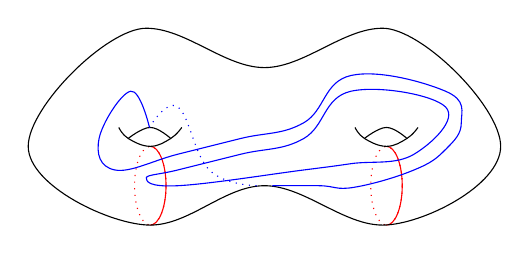
\begin{tikzpicture}


    \begin{scope}[shift={(-0.75,0)}]
    \draw[red,dotted]  (-1.2,-1) ellipse (0.2 and 0.5);
    \clip  (-0.8,-1.6) rectangle (-1.2,0);
    \draw[red]  (-1.2,-1) ellipse (0.2 and 0.5);
    \end{scope}
    
    
    \begin{scope}[shift={(2.25,0)}]
    \draw[red,dotted]  (-1.2,-1) ellipse (0.2 and 0.5);
    \clip  (-0.8,-1.6) rectangle (-1.2,0);
    \draw[red]  (-1.2,-1) ellipse (0.2 and 0.5);\end{scope}
    
    
     \begin{scope}[shift={(4.45,-0.6)}]
        
        \fill[white]  plot[smooth, tension=0.7] coordinates { (-3.68,0.2) (-3.4,0.1) (-3.14,0.2) }  plot[smooth, tension=0.7] coordinates {(-3.68,0.2) (-3.4,0.34) (-3.14,0.2)};
        
        \draw  plot[smooth, tension=0.7] coordinates {(-3.8,0.34) (-3.68,0.2) (-3.4,0.1) (-3.14,0.2) (-3,0.34)};
        \draw  plot[smooth, tension=0.7] coordinates {(-3.68,0.2) (-3.4,0.34) (-3.14,0.2)};
        
        
        
        \end{scope}
        
        
     \begin{scope}[shift={(1.45,-0.6)}]
        
        \fill[white]  plot[smooth, tension=0.7] coordinates { (-3.68,0.2) (-3.4,0.1) (-3.14,0.2) }  plot[smooth, tension=0.7] coordinates {(-3.68,0.2) (-3.4,0.34) (-3.14,0.2)};
        
        \draw  plot[smooth, tension=0.7] coordinates {(-3.8,0.34) (-3.68,0.2) (-3.4,0.1) (-3.14,0.2) (-3,0.34)};
        \draw  plot[smooth, tension=0.7] coordinates {(-3.68,0.2) (-3.4,0.34) (-3.14,0.2)};
        
        
        
        \end{scope}
        
        
    \draw[blue]  plot[smooth cycle, tension=.7] coordinates {(-1.6,-0.8) (-2,-0.9) (-1.6,-1) (0,-0.8) (0.6,-0.72) (1.4,-0.6) (1.8,0) (0.6,0.2) (0,-0.4) (-0.8,-0.6)};
    
    \draw (-2,1) .. controls (-2.5,1) and (-3.5,0) .. (-3.5,-0.5) .. controls (-3.5,-1) and (-2.45,-1.5) .. (-1.95,-1.5) .. controls (-1.45,-1.5) and (-1,-1) .. (-0.5,-1) .. controls (0,-1) and (0.5,-1.5) .. (1,-1.5) .. controls (1.5,-1.5) and (2.5,-1) .. (2.5,-0.5) .. controls (2.5,0) and (1.5,1) .. (1,1) .. controls (0.5,1) and (0,0.5) .. (-0.5,0.5) .. controls (-1,0.5) and (-1.5,1) .. (-2,1);
    \draw[blue]  plot[smooth, tension=.7] coordinates {(-1.96,-0.26) (-2.2,0.2) (-2.6,-0.4) (-2.4,-0.8) (-1.6,-0.6) (-0.8,-0.4) (0,-0.2) (0.6,0.4) (1.8,0.2) (2,-0.2) (1.8,-0.54) (1.4,-0.8) (0.64,-1.02) (0.2,-1) (-0.4,-1)};
    \draw[blue, dotted]  plot[smooth, tension=.7] coordinates {(-0.6,-1) (-1.2,-0.8) (-1.6,0) (-1.96,-0.26)};
    \end{tikzpicture}
    